\section{Durchführung}
\label{sec:Durchführung}
Die Informationen, so wie die Bilder wurden aus den Dokumenten \cite{hin} und \cite{v703} entnommen.
Die Messapparatur wird wie in Abbildung \ref{fig:Schalt} aufgebaut.
Die durch ein einfallendes Teilchen verursachte Ladung $Q$ fließt über den Widerstand $R$ ab und erzeugt einen Spannungsimpuls.
Der Impuls wird über den Kondensator $C$ ausgekoppelt, verstärkt und im Zählgerät registriert oder mit Hilfe eines Oszilloskops sichtbar gemacht.
Für den Versuch wurde eine $\ce{^{204}Tl}$-Quelle genutzt.
Eine Zählrate von $\SI{100}{Imp \per \second}$ wurde nicht überschritten, da dies zur Vermeidung von Totzeit-Korrekturen führt.
\begin{figure}
    \centering
    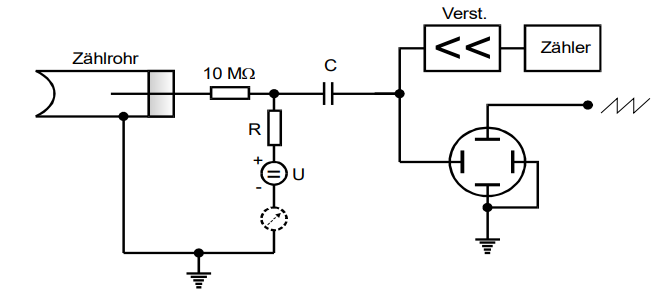
\includegraphics[scale=0.6]{pics/Schalt.png}
    \caption{Skizze der Messapparatur}
    \label{fig:Schalt}
  \end{figure}
\subsection{Aufnahme der Geiger-Müller Charakteristik}
\label{char}
Für die Analyse der Charakteristik wurde die Anzahl der Zerfälle pro Zeitintervall in Schritten von $\symup{\Delta}U=\SI{10}{\volt}$ gemessen.
Die Integrationszeit pro Zählrohrspannung betrug $t=\SI{60}{\second}$, damit die Zählrate im Geiger-Plateau in der Größenordnung von $N=10000\,  \text{Imp}$ liegt.
Da der Fehler mit $\symup{\Delta}N=\sqrt{N}$ gegeben ist und somit für $N=10000$ der Fehler jedes Messpunkts unter $1\% $ liegt.
\subsection{Totzeitbestimmung}
\label{tbes}
Um eine Totzeitkorrektur zu erhalten, wurde die $\ce{^{204}Tl}$-Quelle näher an das Zählrohr gestellt.
Die Messzeit wurde auf $t=\SI{120}{\second}$ erhöht, damit mehr Präzision erzielt werden kann.
Die zwei Quellen wurden wie in Abbildung \ref{fig:zqm} nacheinander positioniert, wonach die Zählraten gemessen wurden.
\begin{figure}
  \centering
  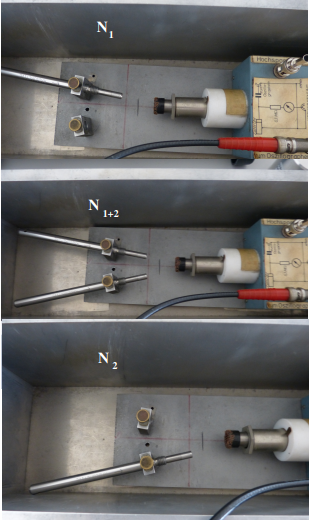
\includegraphics[scale=0.6]{pics/zqmethode.png}
  \caption{Schritte des Zwei-Quellen-Verfahrens}
  \label{fig:zqm}
\end{figure}
Eine weitere Messung wurde mit einem angeschlossenen Oszilloskop durchgeführt. Die Zeitachse wurde auf $\SI{100}{\micro \second \per DIV}$ eingestellt.
\subsection{Bestimmung des Zählrohrstroms}
Der Zählrohrstrom wurde mit dem Amperemeter alle $\SI{50}{\volt}$ abgelesen.